\section{Baseline}
We evaluate our model on the \textsc{SMOL} validation set using BLEURT. This gives us a BLEURT score of $0.689$, by plotting the BLEURT scores on a hexbin plot using bins over the distribution of Cantonese-only characters (see figure \ref{fig:hexbin_baseline}), we can see that the model seems to sometimes perform significantly worse when there are Cantonese-only characters in the sentence. This can be seen more clearly in a violin plot, see figure \ref{fig:violin_baseline}. \todo{validation plot doesnt really show this :-(}

\begin{figure}[H]
    \captionsetup{width=0.45\textwidth}
    \centering
    \begin{minipage}{.5\textwidth}
        \centering
        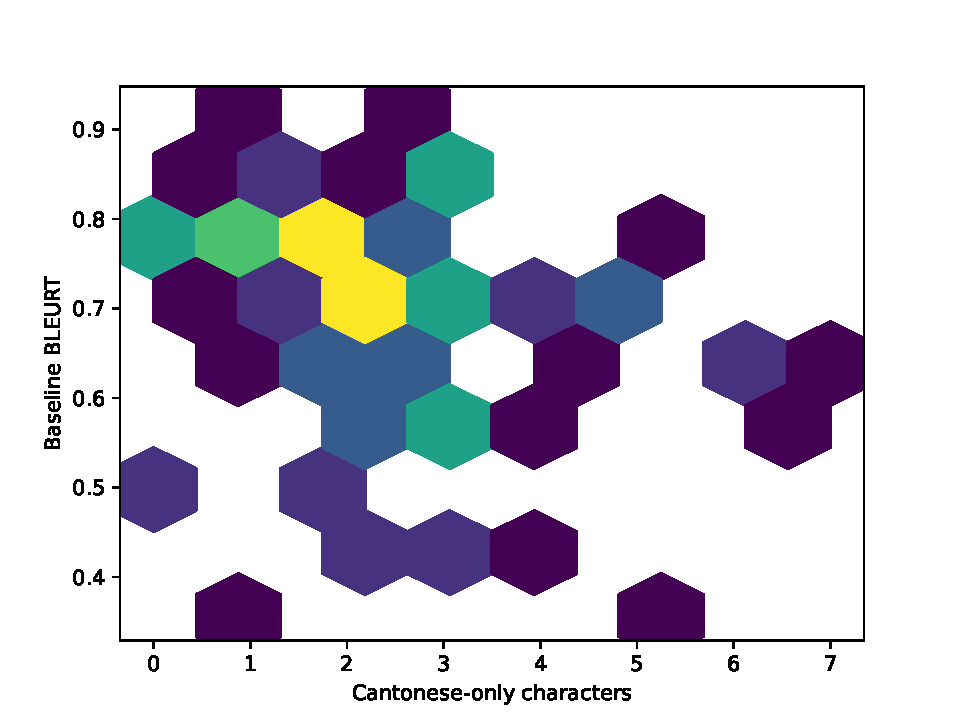
\includegraphics[width=\textwidth]{data_and_figs/hexbin_baseline_validation.pdf}
        \captionof{figure}{Hexbin plot of the BLEURT scores of the baseline model on the validation set. }
        \label{fig:hexbin_baseline}
    \end{minipage}%
    \begin{minipage}{.5\textwidth}
        \centering
        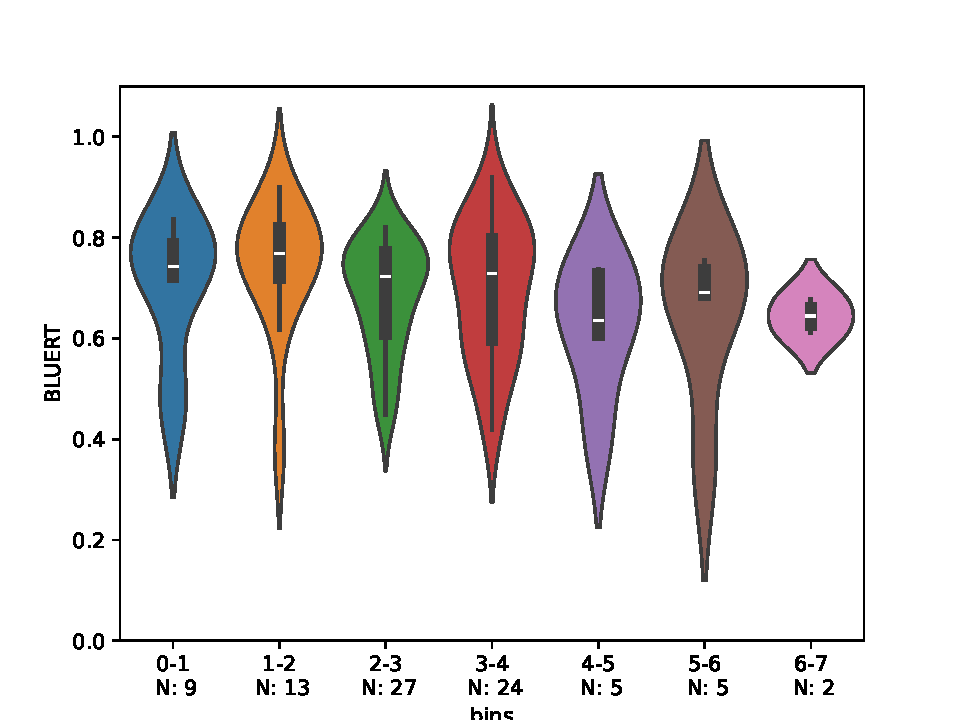
\includegraphics[width=\textwidth]{data_and_figs/violin_baseline_validation.pdf}
        \captionof{figure}{Violin plot of the BLEURT scores of the baseline model on the validation set. }
        \label{fig:violin_baseline}
    \end{minipage}
\end{figure}